\documentclass[a4paper]{article}
\usepackage{labreport}

\begin{document}


\begin{titlepage}
\thispagestyle{fancy} %For the left header
\rhead{}
\chead{}
\lhead{ECGR 2155-Section L94}
\rfoot{}
\cfoot{}
\lfoot{}
\renewcommand{\headrulewidth}{0pt} %Removes horizontal line
    \begin{center}
        \vspace*{1cm}
        
      
       \Large\textbf{University of North Carolina at Charlotte \\[1pt]
	Department of Electrical and Computer Engineering} \\[2pt]
\textit{Laboratory Report 3} \\[5pt]
\textbf{Network Analysis\\[5pt]
Thevenin and Norton Equivalent Circuits\\[5pt]
Time Constant of a RC Circuit\\
}

\noindent\rule{15cm}{0.4pt}
\vfill
        \vspace{0.5cm}
        \textit{Laboratory Experiment Reports 8,9,10} \\
		Author: Patrick Hultberg\\
		Lab Partner: Anthony Grancagnolo	\\
		Date: "12/1/2023" \\
        
        \vspace{1.5cm}
        
        
        
        \vfill
		\vfill
        
       \large This report was submitted in compliance with UNCC POLICY 407\\
THE CODE OF STUDENT ACADEMIC INTEGRITY, Revised November 6, 2014
(http://legal.uncc.edu/policies/up-407) \_\_. (PEH) 
        \vspace{0.8cm}
        
    

    \end{center}
\end{titlepage}


\section{Objectives}

\subsection{Network Analysis}
The objective is to analyze a circuit and measure the real values to validate the calculated values.
\subsection{Thevenin and Norton Equivalent Circuits}
The objective of the lab is to utilize the Thevenin and Norton methods to calculate the current and voltage across any one of several resistors in a circuit and verify the calculated values by measuring the values in the circuits.
\subsection{Time Constant of a RC Circuit}
The objective is to measure the time constant of an RC circuit in order to verify the calculated values.
\section{Equipment List}
\subsection{Network Analysis}

\begin{itemize}
    \item Digital Multimeter
    \item DC Power Supply
    \item Resistors: $470\Omega$, $1K\Omega$ (2), $5.1k\Omega$, $10k\Omega$ 
\end{itemize}

\subsection{Thevenin and Norton Equivalent Circuits}
\begin{itemize}
    \item Digital Multimeter
    \item DC Power Supply
    \item Resistors: $1.2k\Omega$, $3.3k\Omega$, $10k\Omega$
\end{itemize}
\subsection{Time Constant of a RC Circuit}
\begin{itemize}
    \item Digital Multimeter
    \item DC Power Supply
    \item Resistor: $20k\Omega$
    \item Capacitor: $2,200 \mu$F
    \item Alligator (Clips) Jumper
\end{itemize}

\pagebreak
\section{Relevant Theory/Background Information}

\subsection{Network Analysis}
In terms of relevant theory there is a wide variety of methods to calculate the current, voltage, and resistance across a circuit or individual elements. The primary base for all of these methods are Kirchoff's Voltage and Current
laws which show the sum of the currents or voltages across a circuit will equal zero ergo: \\
\[0 = \sum_{i=1}^{n} V_{i}\]\\
and: \\
\[0 = \sum_{i=1}^{n} I_{i}\]\\
With the understanding of Kirchoff's Laws the methods of mesh current analysis, node voltage analysis, and superposition. 
When analysing using mesh current analysis the first step is to break a circuit into meshes which are smaller pieces of a circuit and are functionally the most basic circuit possible.
Then apply Kirchoff's Voltage Law where the voltage across each resistor will be accounted for with Ohm's Law, V = IR, with current in resistors which are located in two loops the currents in each loop must be subtracted. Finally simply solve for each unknown element in each equation.
When analysing using Node Voltage Analysis the first step is to selecting a node as reference or ground. Then use Kirchoff's Current Law for each node and repeat the process described previously.
When utilizing Superposition the first step is to replace all but one current or voltage source with either an open circuit or short circuit respectively. Then apply whatever analysis functions best and repeat the process until all sources have been used. Finally sum all of the current and voltage values to solve for each respectively as seen here:
\[V = \sum_{i=1}^{n} V_{i}\]\\
and here: \\
\[I = \sum_{i=1}^{n} I_{i}\]\\  
\subsection{Thevenin and Norton Equivalent Circuits}
When doing circuit analysis there are occasions when the resistance, voltage, and current at specific terminals and there are two main theorems to conduct these calculations, Thevenin and Norton's theorem. Each theorem abides by Ohm's Law but it is 
focused on the the premise that $R_{Thevenin}$ is equal to $R_{Norton}$ and in the the Ohm's Law equation for these theorems is $V_{oc}$ = $I_{sc}$ * $R_{thevenin}$ or $R_{norton}$. $V_{oc}$ is equal to $V_{thevenin}$ and $I_{sc}$ is equal to $I_{norton}$.
The objective of both theorems is to simplify the circuit to an equivalent resistance , $R_{Thevenin}$ or $R_{Norton}$, and a source, $V_{thevenin}$ with $R_{Thevenin}$ in series or $I_{norton}$ with $R_{Norton}$ in parallel, with a load resistor attached at the terminals. To calculate the previously mentioned equivalent resistance the load resistor must be removed and
"turn off" all the sources in the circuit if all are independent sources and then calculate the resistance. To find $V_{thevenin}$ simply calculate voltage across the resistor parallel to the open circuit using any method preferable to find the open circuit voltage. If given the short circuit current and the resistance $V_{thevenin}$ is simply the multiplication
of these two values. In the case of Norton equivalent cirucits repeat the process to calculate the $R_{Norton}$ then solve for $I_{sc}$ by placing a short circuit across the terminals and calculate the current flowing through the short or solve for $V_{oc}$ and solve for the current using $R_{Norton}$.    

\subsection{Time Constant of a RC Circuit}

The voltage and current change in a capacitor is a natural exponential relationship in the case of charging for voltage the value is found by the expression:
\[V_{c} = V_{S}(1-e^{(-t/\tau)})\]
wherein $\tau$ is equal to equivalent resistance times equivalent capacitence and t is the time passed since the switch which determines when voltage is passing through a capacitor.
Once a steady state is reached at a factor of $\tau$ the change of voltage is no longer significant and that means the capacitor is holding its max charge which is calculated by Q = CV.  
\pagebreak
\section{Experimental Data/Analysis}

\subsection{Network Analysis}

The data below is found by reading the color code nominal value of the resistor and then measure the resistance with the digital multimeter before calculating the percent error 
by subtracting the color code minus the measured value and then dividing that value by the color code value before multiplying by 100 to find the percentage.  

\begin{center}
    \small\textbf{Table 8-1: Resistors Values}
    \begin{tabular}{|p{3 cm}|p{3cm}|p{3 cm}|p{3 cm}|}
        \hline
        Resistance & Measured $(K\Omega)$ & Color Code $(K\Omega)$ & Error (\%) \\
        \hline
        $R_{1}$ & $5.047 k\Omega$ & $5.1k\Omega$ & 1.0392\% \\
        \hline
        $R_{2}$ & $467.5 \Omega$ & $470\Omega$& .5319\% \\
        \hline
        $R_{3}$ & $9.935 k\Omega$ & $10 k\Omega$& .65\% \\
        \hline
        $R_{4}$ & $.999 k\Omega$ & $1 k\Omega$& .1\% \\
        \hline
        $R_{5}$ & $.997 k\Omega$ & $1 k\Omega$ & .3\% \\
        \hline
    \end{tabular}
\end{center}

The table reflects the nominal and measured values and the percent error in the color code which the percent error will be within the tolerance of the the nominal value as denoted by
the color code on the resistor.

To obtain the values in the table below one must use the mesh analysis method to calculate the values for current and then measure the current across each resistor. In order to get the 
percent error simply subtract the calculated amperage minus the measured amperage and divide by the calculated value before multiplying by 100.

\begin{center}
    \small\textbf{Table 8-2: Mesh Currents}
    \begin{tabular}{|p{3 cm}|p{3cm}|p{3 cm}|p{3 cm}|}
        \hline
        Current & Measured (mA) & Calculated (mA) & Error (\%) \\
        \hline
        $I_{A}$ & .806 mA & .813 mA & .861\%  \\
        \hline
        $I_{B}$ & .043 mA & .0404 mA & 5.581\% \\
        \hline
        $I_{C}$ & .910 mA & .913 mA & .329\% \\
        \hline
    \end{tabular}
\end{center}

The calculated and measured values are different due to the assumptions that the calculated amperage which are the resistor values are the nominal values without the 
tolerance and there all conditions of the circuit are ideal.

To find the values in the table below utilize the various methods of analysis for the voltage across each resistor then measure the voltage across each resistor. To find the 
simulation values set up the circuit as shown in figure 8-1 in Matlab then add the ampmeters in series with each resistor as done in the lab and the voltmeters 
in parallel with each resistor and the readings of both sets of meters will be the simulation values which is shown in Figure 8-2.
\vspace{.5 cm}
\begin{center}
    \begin{figure}[H]\label{fig8-2}
        \begin{center}
            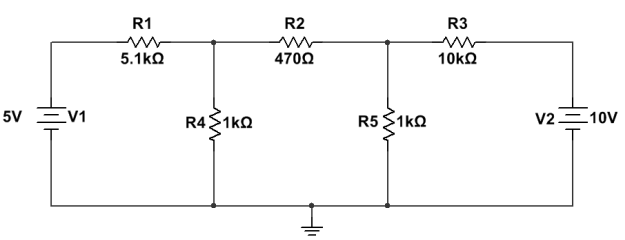
\includegraphics[width = 16 cm]{fig8-1}\\
            \small\textbf{Figure 8-1: Circuit for experiment 8}\\    
        \end{center}
    \end{figure}
\end{center}

\begin{center}
    \small\textbf{Table 8-3: Resistors Voltages}
    \begin{tabular}{|p{2 cm}|p{2cm}|p{2 cm}|p{2 cm}|p{2 cm}|p{2 cm}|}
        \hline
         & Measured & Mesh Method & Nodal Analysis & Superposition & Simulation \\
        \hline
        $V_{R1}$ & 4.14 V & 4.1463 V & 4.43368 V & 4.1466 V & 4.147 V \\
        \hline
        $V_{R2}$ & .021 V & .018988 V & .018 V & .01897 V & .01897 V \\
        \hline
        $V_{R3}$ & 9.123 V & 9.13 V & 9.128 V & 9.158 V & 9.128 V \\
        \hline
        $V_{R4}$ & .852 V & .854 V & .853 V & .853 V & .8534 V \\
        \hline
        $V_{R5}$ & .873 V & .8721 V & .872 V & .873 V & .8724 V \\
        \hline
    \end{tabular}
\end{center}

The data in the table above displays the most accurate method to analyze voltage in a circuit is superposition as in the majority of all cases in the circuit it has the least error in the 
value when compared to the measured values.

To obtain the data in the table below repeat the process described for the previous table however instead of solving for voltage solve for the current running through each resistor.

\begin{center}
    \small\textbf{Table 8-4: Resistors Current}
    \begin{tabular}{|p{2 cm}|p{2cm}|p{2 cm}|p{2 cm}|p{2 cm}|p{2 cm}|}
        \hline
         & Measured & Mesh Method & Nodal Analysis & Superposition & Simulation \\
        \hline
        $I_{R1}$ & .803 mA  & .813 mA & .8131 mA & .81305 mA & .8131 mA \\
        \hline
        $I_{R2}$ & .043 mA & .0406 mA & .0404 mA & .04037 mA  & .04034 mA \\
        \hline
        $I_{R3}$ & .911 mA & .913 mA & .9128 mA & .91276 mA & .9128 mA \\
        \hline
        $I_{R4}$ &.825 mA & .8536 mA & .853 mA &  .853 mA & .8534 mA \\
        \hline
        $I_{R5}$ & .834 mA & .8271 mA & .872 mA & .873 mA & .8724 mA\\
        \hline
    \end{tabular}
\end{center}

The data in the table above displays that in most cases the most accurate method to calculate the current across a resistor which is in parallel to the power supplies
is mesh analysis and the most accurate method to measure resistors in series is nodal analysis.

The figure below is the simulated circuit in Figure 8-1 which was constructed in MatLab's Similink environment which the ampmeters are in series with the resistor being measured and the voltmeters in parallel 
with the resistor being measured.

\begin{center}
    \begin{figure}[H]\label{fig8-2}
        \begin{center}
            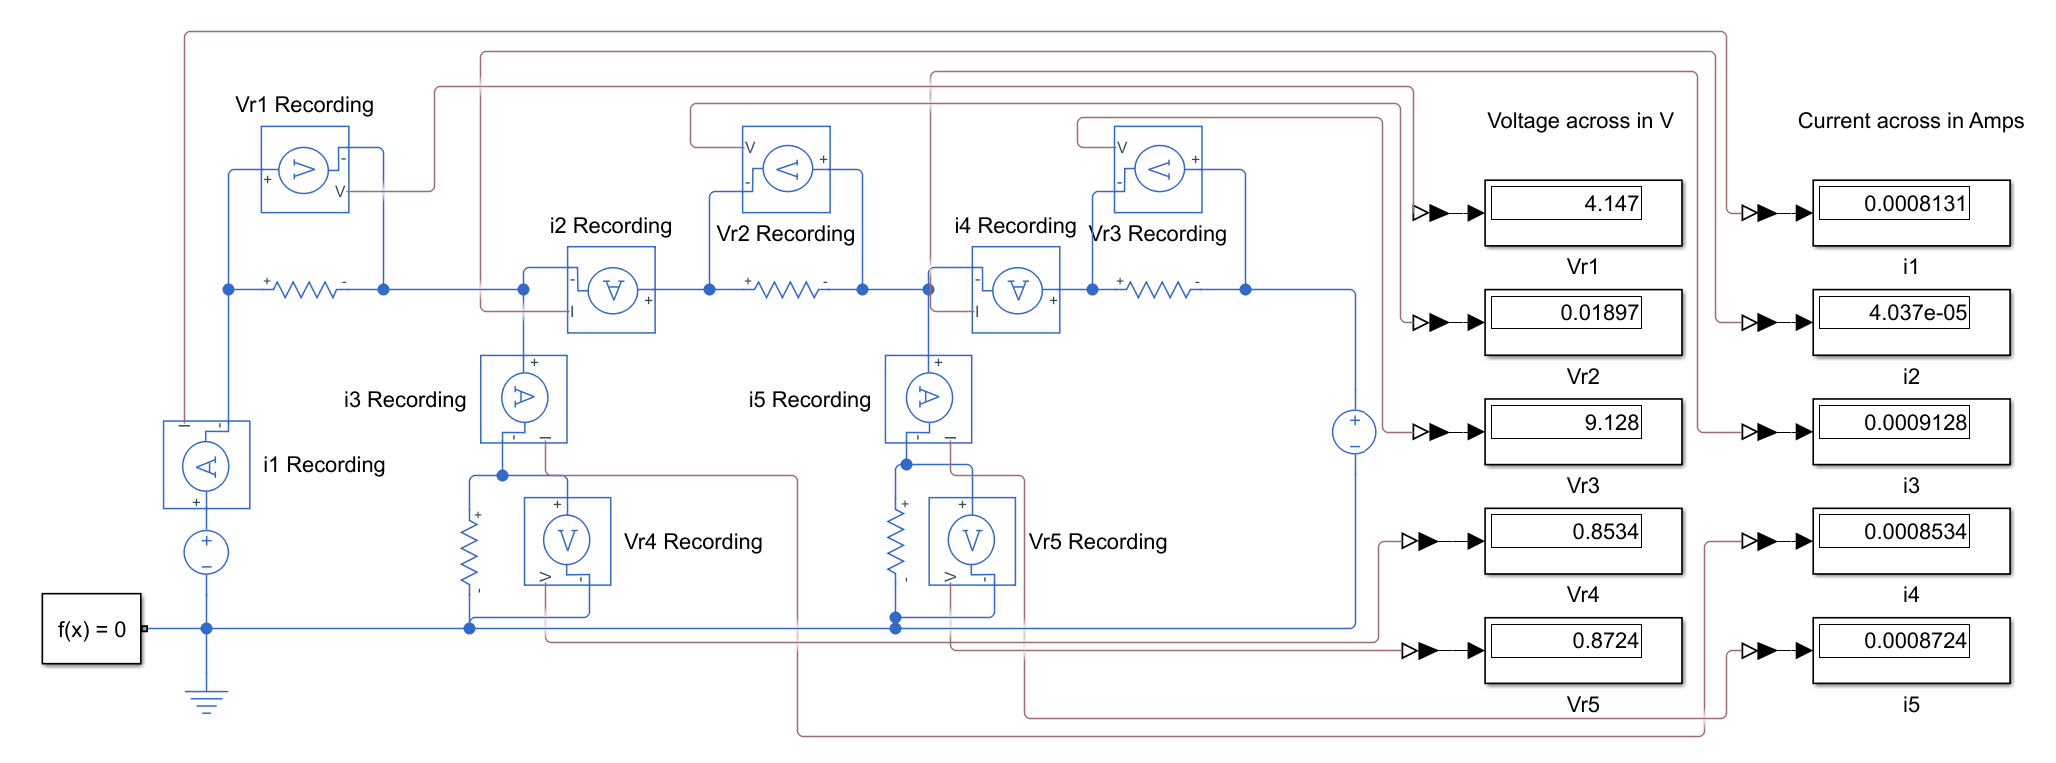
\includegraphics[width = 16 cm]{Figure_8-1}\\
            \small\textbf{Figure 8-2: Simulated model of the circuit in Figure 8-1}\\    
        \end{center}
    \end{figure}
\end{center}

The measurements in the figure is the simulated values in the previous tables after running the simulation of the circuit.
\pagebreak

 

\subsection{Thevenin and Norton Equivalent Circuits}

To obtain the values in the table below the current through the load resistor and voltage across the load resistor for the thevenin and norton equivalent circuits
which can be obtained by calculating the thevenin and norton equivalent resistance, the norton current, and the thevenin voltage. Then plug in the load resistor then using 
current and voltage division to calculate the values in the table below.


\begin{center}
    \small\textbf{Table 9-1: Calculated Voltage and Current for Resistor R3}
    \begin{tabular}{|p{3 cm}|p{3cm}|p{3 cm}|}
        \hline
         & Thevenin Equivalent & Norton Equivalent\\
        \hline
        $I_{R3}$ & 4.9 mA & 4.9 mA  \\
        \hline
        $V_{R3}$ & 16.17 V & 16.17 V  \\
        \hline
        
    \end{tabular}
\end{center}

The values in the table above display the theoretical values of the thevenin and current equivalents of the circuit.

The values in the table below are found by constructed in Figure 9-1 but remove the load resistor and replace it with a multimeter then measure the voltage across the unconnected leads to find the thevenin voltage and the short circuit 
currents across the same leads to find the norton current.

\begin{center}
    \begin{figure}[H]\label{fig9-3}
        \begin{center}
            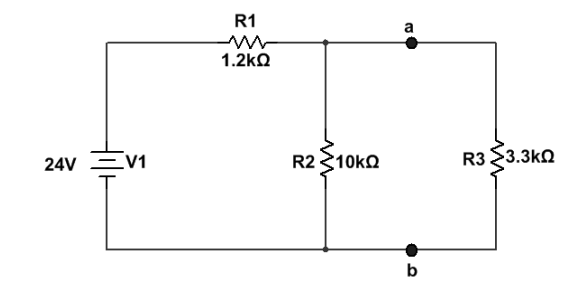
\includegraphics[width = 8cm]{Fig9-3}\\
            \small\textbf{Figure 9-1: Circuit for Thevenin and Norton Analysis}
        \end{center}
    \end{figure}
\end{center}

\begin{center}
    \small\textbf{Table 9-2: Measured Thevenin and Norton Equivalents}
    \begin{tabular}{|p{3 cm}|p{3cm}|p{3 cm}|p{3 cm}|}      
        \hline
        \multicolumn{2}{|c|}{Thevenin Equivalent} & \multicolumn{2}{|c|}{Norton Equivalent}  \\
        \hline
        $v_{TH}$ & 21.43 V & $i_{N}$ & 18.3 mA \\
        \hline
        $R_{TH}$ & $1.056k\Omega$ & $R_{N}$ & $1.056k\Omega$ \\
        \hline
    \end{tabular}
\end{center}

The data in the table above displays the values measured for the thevenin and norton equivalent circuits and displays the values for $R_{TH}$ and $R_{N}$ are the same and the current, resistance, and voltage are linked using Ohm's Law.  

The data in the table below is found using the same circuit as in figure 9-1 but leaving the load resistor attached rather than replacing it with a multimeter then measure the current and voltage across the load resistor. 

\begin{center}
    \small\textbf{Table 9-3: Measured Voltage and Current for Resistor R3}
    \begin{tabular}{|p{3 cm}|p{3 cm}|p{3 cm}|p{3 cm}|}
        \hline
        & Figure 9-3 & Thevenin Equivalent & Norton Equivalent \\
        \hline
        $I_{R3}$ & 4.961 mA & 4.961 mA & 4.596 mA \\
        \hline
        $V_{R3}$ & 16.19 V & 16.18 V & 15 V\\
        \hline
    \end{tabular}
\end{center}

The data in the table above which is close to the calculated values but different due to the calculation assuming ideal conditions and no tolerance which in the measured values exist.

\pagebreak
\subsection{Time Constant of a RC Circuit}

To obtain the values in the table below first calculate the time constant and 5 times the time constant which is the equivalent resistance times equivalent capacitence. Then constrcut the circuit in figure 10-1.
Then measure the current in the circuit every 15 seconds and the intial current. Repeat the proces in the last step again then average the measurements of the two trials and use that current value to calculate the voltage across the resistor and the capacitor.

\begin{figure}[H]\label{fig10-1}
    \begin{center}
        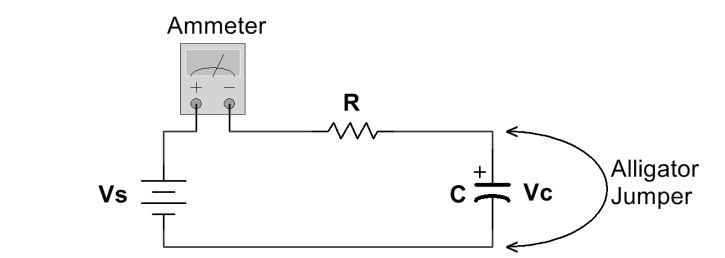
\includegraphics[width = 7 cm]{fig10-1}\\
        \small\textbf{Figure 10-1 Series RC Circuit for Experimental Setup}
    \end{center}
\end{figure} 

\begin{center}
    $\tau$ = 44 seconds  Initial Current = 1.745 mA  \\
    5$\tau$ =  220 seconds \\
    \small\textbf{Table 10-1: Data Table for RC Time Constant}\\
    \begin{tabular}{|p{2 cm}|p{2 cm}|p{2 cm}|p {2 cm}|p {2 cm}|p{2 cm}|}
        \hline
        Time (min:sec) & \multicolumn{3}{|c|}{Current (mA)} & Resistor Voltage (V) & Capacitor Voltage (V) \\
        \hline
        & Trial 1 & Trial 2 & Average & & \\
        \hline
        0:00 & 1.745 mA & 1.745 mA & 1.745 mA & 34.9 V  & 0 V \\
        \hline
        0:15 & 1.242 mA & 1.24 mA & 1.241 mA & 24.82 V & 10.08 V \\
        \hline
        0:30 & .901 mA & .900 mA & .9005 mA & 18.01 V &  16.86 V \\
        \hline
        0:45 $\tau$ & .662 mA & .666 mA & .664 mA & 13.28 V & 21.62 V \\
        \hline
        1:00 & .490 mA & .500 mA & .495 mA & 9.9 V & 25 V \\
        \hline
        1:15 & .365 mA & .373 mA & .369 mA & 7.38 V & 27.52 V \\
        \hline
        1:30 & .277 mA & .274 mA & .2755 mA & 5.51 V & 29.39 V \\
        \hline
        1:45 & .212 mA & .207 mA & .2095 mA & 4.19 V & 30.71 V \\
        \hline
        2:00 & .165 mA & .158 mA & .1615 mA & 3.23 V & 31.67 V \\
        \hline
        2:15 & .125 mA & .112 mA & .1185 mA & 2.37 V & 32.53 V \\
        \hline
        2:30 & .100 mA & .092 mA & .096 mA & 1.92 V & 32.98 V \\
        \hline
        2:45 & .076 mA & .072 mA & .074 mA & 1.48 V & 33.42 V \\
        \hline
        3:00 & .062 mA & .057 mA & .0595 mA & 1.19 V & 33.71 V \\
        \hline
        3:15 & .050 mA & .045 mA & .0475 mA & .95 V & 33.95 V \\
        \hline
        3:30 & .041 mA & .036 mA & .0385 mA & .77 V & 34.13 V \\
        \hline
        3:45 & .034 mA & .029 mA & .0315 mA & .63 V & 34.27 V \\
        \hline
        4:00 & .028 mA & .024 mA & .026 mA & .52 V & 34.38 V \\
        \hline
        4:15 & .023 mA & .020 mA & .0215 mA & .43 V & 34.47 V \\
        \hline
        4:30 & .020 mA & .016 mA & .018 mA & .36 V & 34.54 V \\
        \hline
        4:45 5$\tau$ & .017 mA & .014 mA & .0155 mA & .31 V & 34.59 V \\
        \hline
        5:00 & .015 mA & .012 mA & .0135 mA & .27 V & 34.63 V \\
        \hline
        5:15 & .013 mA & .010 mA & .0115 mA & .23 V & 34.67 V \\
        \hline
        5:30 & .011 mA & .009 mA & .010 mA & .2 V & 34.7 V \\
        \hline
        5:45 & .010 mA & .008 mA & .009 mA & .18 V & 34.72 V \\
        \hline
        6:00 & .009 mA & .007 mA & .008 mA & .16 V & 34.74 V \\
        \hline
    \end{tabular}
\end{center}

The data in the table above displays as time passes and the capacitor reaches the steady state there will be less current in the circuit then less voltage across the resistor due to the constant resistance and the current decreasing the voltage will decrease.
Furthermore, since the voltage in the circuit is constant as the voltage across the resistor decreases the voltage in the capacitor will increase until it reaches its steady state.

\section{Conclusions}

\subsection{Network Analysis}

Each method of calculation will introduce error due to its assumption of ideal conditions. Furthermore, each almost all methods of calculations
will give similar value but will vary in precision.

\subsection{Thevenin and Norton Equivalent Circuits}

Thevenin and Norton equivalent circuits are way to reduce circuits to a simpler form that makes finding current though, voltage in, and resistance in a circuit. The Norton Current and Thevenin Voltage
will be the values across the load resistor. Norton Resistance equals Thevenin Resistance and the Thevenin Voltage is equal to the Thevenin Resistance times the Norton Current.  

\subsection{Time Constant of a RC Circuit}

As a capacitor is charged current will decrease until the capacitor is fully charged thus making an open circuit. Furthermore, the voltage will be collected into the capacitor as the voltage across the resistor goes down.

\pagebreak
\section{Post Lab}

\subsection{Network Analysis}

\begin{enumerate}
    \item From the data obtained in this experiment, calculations and simulations; discuss on the validity of Mesh Analysis, Nodal Analysis, and superposition.\\
    Depending on the precision required to measure the voltage and current will result in each method being more or less accurate. Those which require more precision in the measure of voltage will mean that the 
    the node method is more accurate whereas in the case of current the loop method is more acurrate.
\end{enumerate}
    

\subsection{Thevenin and Norton Equivalent Circuits}

\begin{enumerate}
    \item From the data obtained in this experiment and prelab calculations simulations; discuss on\\
    \begin{enumerate}
        \item Observations regarding the current through resistor R3.\\
        The current through resistor R3 is equal to 4.961 mA which is equivalent to the Thevenin equivalent current based of the Ohm's Law calculations and is higher than the Norton equivalent current, 4.596; however, this is down to fluctuation due to the shorting of the power supply.
        \item Observations regarding the voltage across resistor R3.\\
        The same can be said of the voltage across R3 for similar reasons as observed in the current across the same resistor and due to Ohm's Law with resistance is constant the current fluctuates meaning the voltage will fluctuate. 
        \item Observations regarding the Thevenin equivalent.\\
        The Thevenin equivalent is larger than the voltage across the load resistor this is down to the fact the current is concentrated in the circuit with out being divided across the two resistors proportionally thus meaning a higher value for voltage with resistance remaining constant.
        \item Observations regarding the Norton equivalent.\\
        The Norton equivalent is also much higher than the current across R3 because the resistance in a short circuit is far smaller or non existant when compared the resistance across the resistor.  
    \end{enumerate}
\end{enumerate}

\subsection{Time Constant of a RC Circuit}

\begin{enumerate}
    \item From the data obtained in this experiment in a single graph; \\
    \begin{enumerate}
        \pagebreak
        \item Plot $V_{R}$ vs. time \\
        \begin{center}
            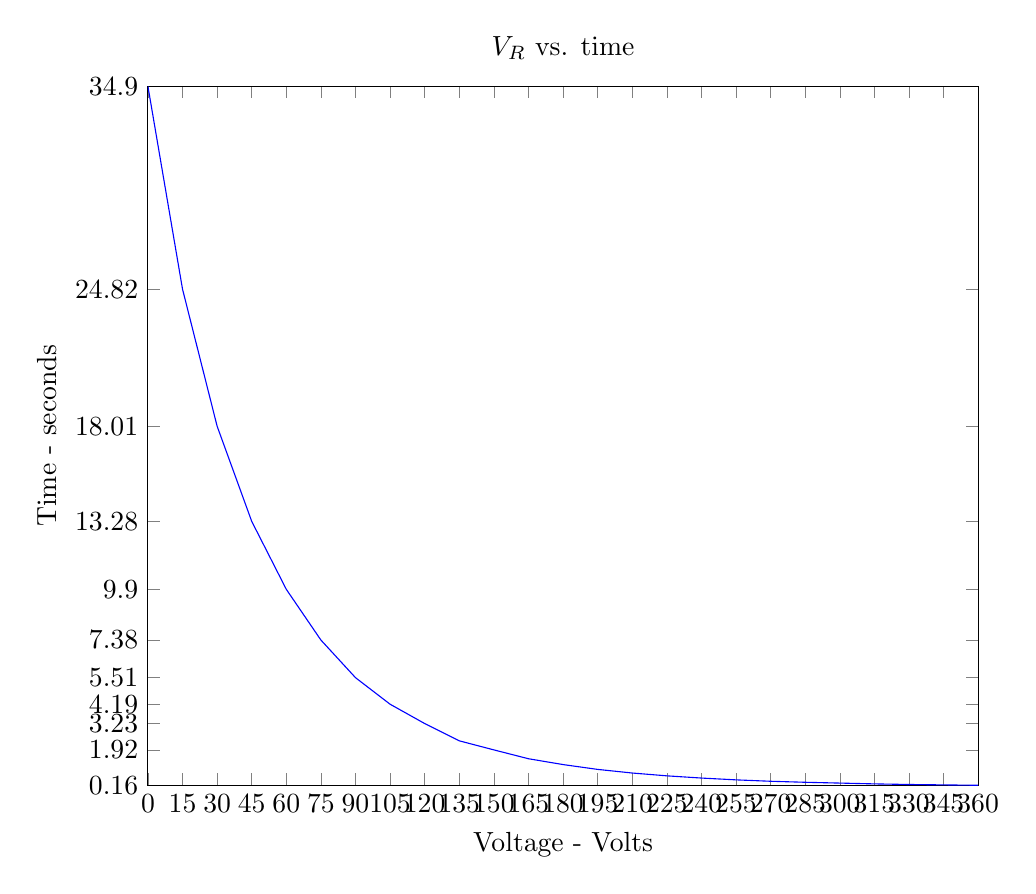
\begin{tikzpicture}
                \begin{axis}
                    [
                    title ={$V_{R}$ vs. time},
                    xlabel = {Voltage - Volts},
                    ylabel = {Time - seconds},
                    xmin=0, xmax=360,
                    ymin=.16, ymax=34.9,
                    width=\textwidth,
                    xtick={0,15,30,45,60,75,90,105,120,135,150,165,180,195,210,225,240,255,270,285,300,315,330,345,360},
                    ytick={.16,1.92,3.23,4.19,5.51,7.38,9.9,13.28,18.01,24.82,34.9},
                    ]
                    \addplot[
                        color=blue,
                    ]
                    coordinates{ 
                    (0,34.9)
                    (15,24.82)
                    (30,18.01)
                    (45,13.28)
                    (60,9.9)
                    (75,7.38)
                    (90,5.51)
                    (105,4.19)
                    (120,3.23)
                    (135,2.37)
                    (150,1.92)
                    (165,1.48)
                    (180,1.19)
                    (195,.95)
                    (210,.77)
                    (225,.63)
                    (240,.52)
                    (255,.43)
                    (270,.36)
                    (285,.31)
                    (300,.27)
                    (315,.23)
                    (330,.2)
                    (345,.18)
                    (360,.16)};
                \end{axis}
            \end{tikzpicture}
        \end{center}
        \pagebreak
        \item Plot $V_{c}$ vs. time \\
        \begin{center}
            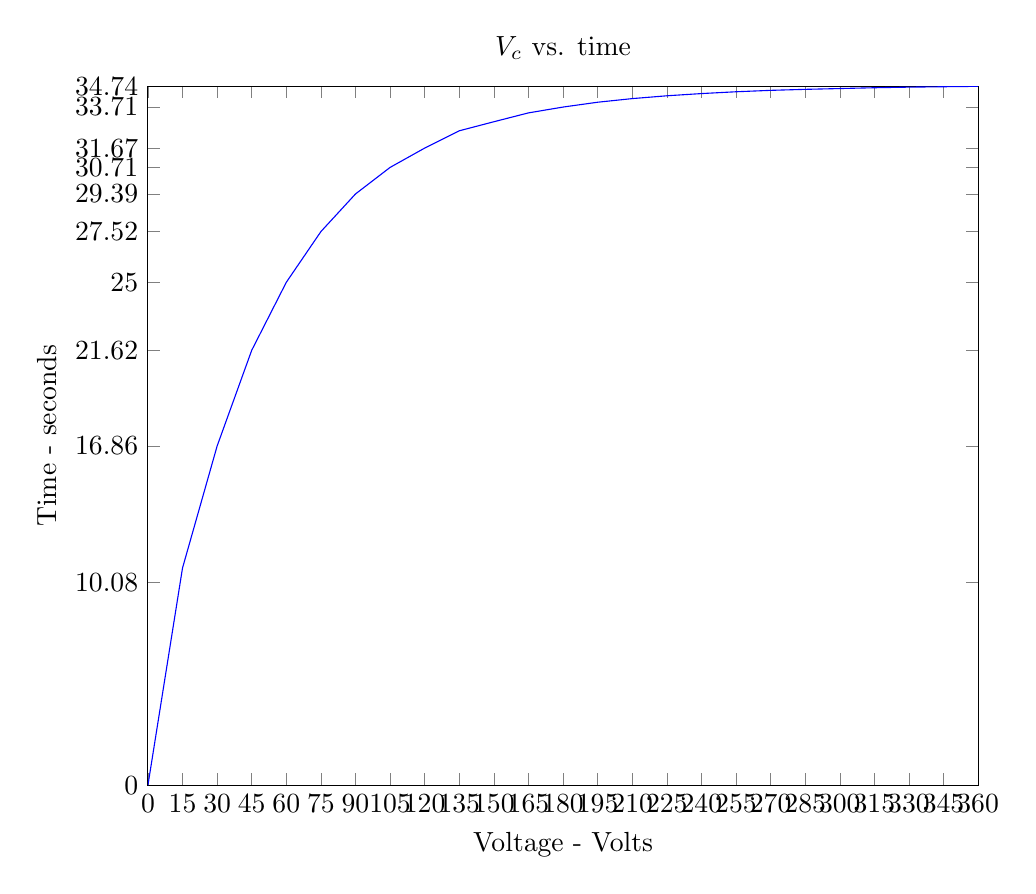
\begin{tikzpicture}
                \begin{axis}
                    [
                    title ={$V_{c}$ vs. time},
                    xlabel = {Voltage - Volts},
                    ylabel = {Time - seconds},
                    xmin=0, xmax=360,
                    ymin=0, ymax=34.74,
                    width=\textwidth,
                    xtick={0,15,30,45,60,75,90,105,120,135,150,165,180,195,210,225,240,255,270,285,300,315,330,345,360},
                    ytick={0,10.08,16.86,21.62,25,27.52,29.39,30.71,31.67,33.71,34.74},
                    ]
                    \addplot[
                        color=blue,
                    ]
                    coordinates{ 
                    (0,0)
                    (15,10.8)
                    (30,16.86)
                    (45,21.62)
                    (60,25)
                    (75,27.52)
                    (90,29.39)
                    (105,30.71)
                    (120,31.67)
                    (135,32.53)
                    (150,32.98)
                    (165,33.42)
                    (180,33.71)
                    (195,33.95)
                    (210,34.13)
                    (225,34.27)
                    (240,34.38)
                    (255,34.47)
                    (270,34.54)
                    (285,34.59)
                    (300,34.63)
                    (315,34.67)
                    (330,34.7)
                    (345,34.72)
                    (360,34.74)};
                \end{axis}
            \end{tikzpicture}
        \end{center}
    \end{enumerate}
    \item After the graphs have been completed, do the following: \\
    \begin{enumerate}
        \item Describe the capacitor voltage behavior from 0 through $5\tau$, in terms of initial and final voltage magnitude, linearity and rate of change. \\
        The initial voltage is 0.16 V while the final voltage at 5$\tau$ is 34.59 V which the rate of change is a positive exponential curve.
        \item Describe the resistor voltage behavior from 0 through $5\tau$, in terms of initial and final voltage magnitude, linearity and rate of change. \\
        The intial voltage is 34.9 V and the final voltage at 5$\tau$ is 0.31 V and the rate of change is a negative exponential curve.
        \item To how many volts has $V_{c}$ charged in one time constant? \\
        21.62 V
        \item To what \% has the capacitor charged to at this point? \\
        37.77\%
        \item Using the equation in the introduction section of this experiment, show the calculation of $V_{C}$ for a time equal to one time constant. \\
        \[22.12 = 35(1-e^{-1})\]
        \item How many volts are across the resistor at the end of one time constant? What \% is this of the total possible voltage change? \\
        13.28 V and 28.55\%
        \item From the graphs read the values of capacitor and resistor voltage at 4 minutes. \\
        $V_{(R)}$ = .52 V and $V_{(c)}$ = 34.38 V
        \item Calculate the values of capacitor and resistor voltage at 4 minutes. \\
        \[34.85 = 35(1-e^{(-240/44)})\]
        \item From the results of g and h above, what do you conclude about the accuracy of your graphs? \\
        They approximately accurate because the sum of the voltage in the circuit is 34.9 V which is .05 V more than the estimated voltage in the capacitor the approximate difference in the capicitor voltage is due to the resistor causing a voltage drop prior to the capacitor. 
    \end{enumerate}
\end{enumerate}

\end{document}